\section{Algorithms for Data Flow Analysis}


\begin{frame}
  \frametitle{Program Analysis\footnote{Pedro Costa and Luis Amaral contributed to these slides}}

  \begin{block}{Goal}
    Predict {\color{blue}safe} and {\color{blue}computable approximations} of the possible
    behaviours that arise at runtime when executing a program. \pause \\
    Usage Scenarios:
    \begin{itemize}
     \item program optimization
     \item program transformation
     \item program design metrics
     \item software security
    \end{itemize}
  \end{block}
\end{frame}

\begin{frame}
  \frametitle{The While Language}

  \begin{block}{Features}
    \begin{itemize}
     \item tiny (imperative) programming language
     \item integer and boolean expressions  
     \item conditionals and loops \pause
     \item every statement has a unique label  
    \end{itemize}
  \end{block}

\end{frame}

\begin{frame}
  \frametitle{An introduction to DataFlow Analysis}

  \begin{enumerate}
    \item The program is modeled as a (control-flow) graph: the nodes are the
  the elementary blocks (statements) and the edges describe how the
  control might pass from one statement to another.

    \item We define functions for every node, so that data flow information
      can be computed using pairs of \emph{Gen} and \emph{Kill} functions---considering the
      information produced in the previou(s) node(s). 
  \end{enumerate}

  \pause Computing a solution for a dataflow problem often
  requires multiple iteractions, where every new iteration
  provides a better approximation (monotone framework).
  The iteration continues until achieving a {\color{blue}fixpoint}.
  \pause $f(s) = s$
  
\end{frame}

\begin{frame}[fragile]
  \frametitle{Running Example}
  
  \begin{center}
  	\large Example 01: Factorial
  \end{center}
  
  \begin{columns}
    \column[t]{0.40\textwidth}
While language
    
\begin{verbatim}
y := x;           (1)
z := 1;           (2)
while(y > 1) do   (3)
  z := z * y;     (4) 
  y := y - 1;     (5) 
y := 0;           (6) 
\end{verbatim}
\column[t]{0.60\textwidth}
\pause Control Flow Graph
\digraph[scale=0.40]{cfg01}{
  node [fontname = "Handlee"];
  edge [fontname = "Handlee"];

  n1 [
    label = "y := x";
    shape = rect;
    xlabel="1";
  ];
  n2 [
    label = "z := 1";
    shape = rect;
    xlabel="2";
  ];
  n3 [
    label = "while y > 1";
    shape = diamond;
    xlabel="3";
  ];
  n4 [
    label = "z := z * y";
    shape = rect;
    xlabel="4";
  ];
  n5 [
    label = "y := y - 1";
    shape = rect;
    xlabel="5";
  ];
  n6 [
    label = "y := 0"; 
    shape = rect;
    xlabel="6";
  ]; 
  n1 -> n2;
  n2 -> n3;
  n3 -> n4[label = "yes"]
  n4 -> n5; 
  n5 -> n3; 
  n3 -> n6 [label = "no"];
  
  {
    rank=same;
    n3;n4;
  }
}

\end{columns}
\end{frame}


\subsection{Reaching Definitions}

\begin{frame}
  \begin{huge}
    Reaching Definitions
  \end{huge}
  \pause

  \vskip+1.5em
  
  \begin{itemize}
   \item Application in different areas, including {\color{blue}tainted analysis}.
   \item Allows the construction of \emph{def-use} and \emph{use-def} chains. These
     chains facilitate several transformations targeting program optimization. 
  \end{itemize}
\end{frame}

\begin{frame}
  \frametitle{Reaching Definitions Algorithm}

  \begin{block}{Informal definition}
   For every vertice \texttt{(from, to)} in the control flow,
   we check if \texttt{assignment(v, exp) := to} holds (\texttt{to} is
   an assignment).\pause If this is the case, we remove all definitions that
   assign a value to \texttt{v} ({\color{blue}Kill}) from the input set, and expose a new
   definition of \texttt{v} at statement \texttt{to} ({\color{blue}Gen}).
   If \texttt{to} is not a definition (an assignment), than we just propagate the
   sets of definitions that arrive at \texttt{to}.
  \end{block} 
\end{frame}

\begin{frame}{Equations for Reaching Definitions}
  \centering{
    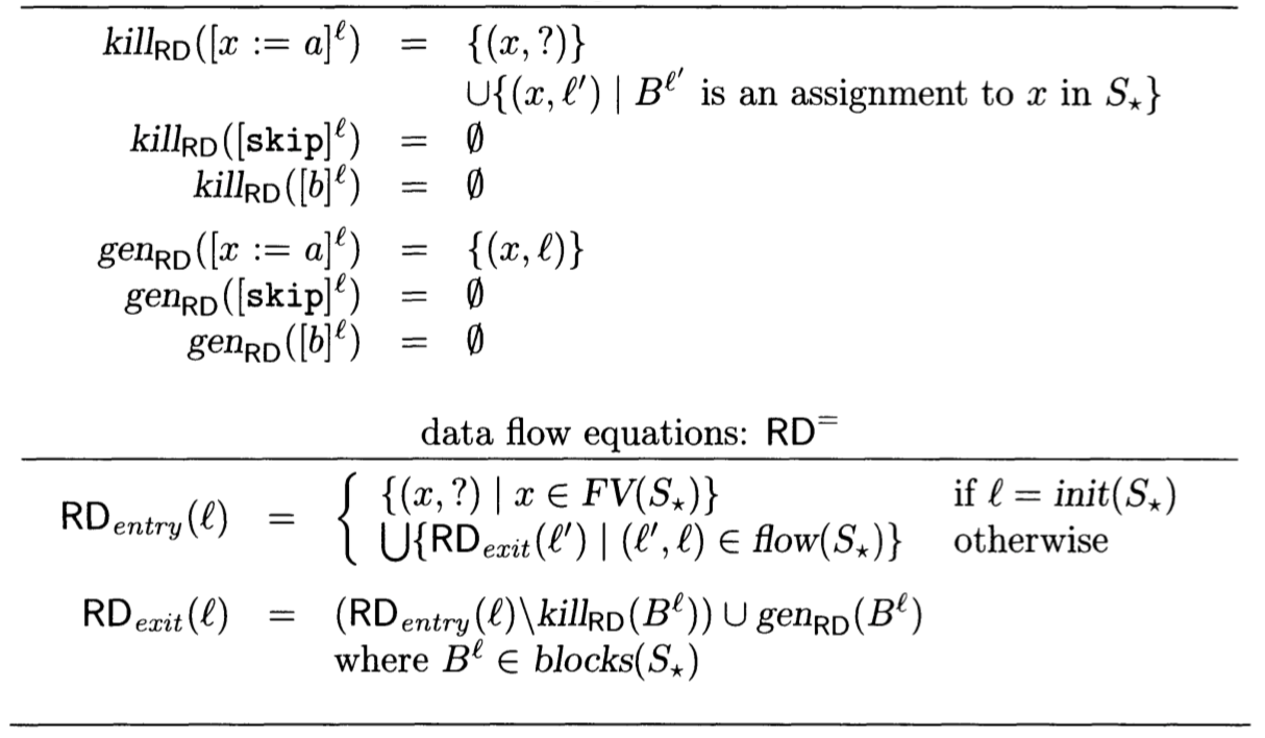
\includegraphics[scale=0.5]{images/rde}

    \scriptsize{Nielson et al. Principles of Program Analysis. Springer-Verlag. 2005}
  }
\end{frame}

\begin{frame}[fragile]
  \frametitle{Iterative Reaching Definitions Algorithm}

  \begin{block}{Equations}
    \begin{itemize}
    \item $Out(s) = Gen(s) \cup (In(s) - Kill(s))$  
    \item $In(s) = \bigcup_p Out(p), p \in pred(s), s \in stmts$
    \end{itemize}
  \end{block}

  \pause

\begin{block}{Iterative algorithm}
  \begin{algorithmic}
    \Procedure{ReachingDefinitions}{CFG}
     \State $Out[Start] = \{\}$ 
     \For{$s \leftarrow CFG.V$}
       \State{$Out[s] = \{ \}$}
     \EndFor
     \While{$\text{not fixed}$}
       \For{$s \leftarrow CFG.V$}
         \State{$\text{compute In[s]}$}
         \State{$\text{compute Out[s]}$}
       \EndFor
     \EndWhile
    \State {\bf return} $(In, Out)$
    \EndProcedure 
  \end{algorithmic}
\end{block}
\end{frame}



%%%%%%%%%%%%%%%%%%%%%%%%%%%%%%%%%%%%%%%%%%%%%%%%%%%%%%%%%
\begin{frame}[fragile, t]
 \frametitle{Iteration 1} 

\begin{center}
\begin{scriptsize}
\begin{minipage}{8cm}
    \begin{block}{Equations}
    \begin{itemize}
        \item $Out(s) = Gen(s) \cup (In(s) - Kill(s))$  
	    \item $In(s) = \bigcup_p Out(p), p \in pred(s), s \in stmts$
    \end{itemize}
    \end{block}
\end{minipage}
\end{scriptsize}
\end{center}

\begin{columns}[T]
\begin{column}[T]{.4\textwidth}
    \vspace{0pt}
    \digraph[scale=0.40]{cfg01}{
  node [fontname = "Handlee"];
  edge [fontname = "Handlee"];

  n1 [
    label = "y := x";
    shape = rect;
    xlabel="1";
  ];
  n2 [
    label = "z := 1";
    shape = rect;
    xlabel="2";
  ];
  n3 [
    label = "while y > 1";
    shape = diamond;
    xlabel="3";
  ];
  n4 [
    label = "z := z * y";
    shape = rect;
    xlabel="4";
  ];
  n5 [
    label = "y := y - 1";
    shape = rect;
    xlabel="5";
  ];
  n6 [
    label = "y := 0"; 
    shape = rect;
    xlabel="6";
  ]; 
  n1 -> n2;
  n2 -> n3;
  n3 -> n4[label = "yes"]
  n4 -> n5; 
  n5 -> n3; 
  n3 -> n6 [label = "no"];
  
  {
    rank=same;
    n3;n4;
  }
}

    \end{column}
    \begin{column}[T]{.6\textwidth}
\vspace{30pt}    
	\begin{scriptsize}
	   \begin{table}[]
\begin{tabular}{|l|l|l|}
\hline
n & IN{[}n{]} & OUT{[}n{]} \\ \hline
1  & \pause \{ \}            & \pause \{(y,1)\} \\ \hline
2  & \pause \{(y,1)\}        & \pause \{(y,1), (z,2)\} \\ \hline
3  & \pause \{(y,1), (z,2)\} & \pause \{(y,1), (z,2)\} \\ \hline
4  & \pause \{(y,1), (z,2)\} & \pause \{(y,1), (z,4)\} \\ \hline
5  & \pause \{(y,1), (z,4)\} & \pause \{(y,5), (z,4)\} \\ \hline
6  & \pause \{(y,1), (z,2)\} & \pause \{(y,6), (z,2)\} \\ \hline
\end{tabular}
\end{table}   
	\end{scriptsize}
	\end{column}
%\hfill
    
\end{columns}

\end{frame}



%%%%%%%%%%%%%%%%%%%%%%%%%%%%%%%%%%%%%%%%%%%%%%%%%%%%%%%%%
\begin{frame}[fragile, t]
	\frametitle{Iteration 2} 
	
	\vspace{-1cm}
	
	\begin{columns}[T]
		\begin{column}[T]{.4\textwidth}
	\begin{center}
		\begin{scriptsize}
			\begin{minipage}{8cm}
		%		\begin{block}{Equations}
					\begin{itemize}
						\item $Out(s) = Gen(s) \cup (In(s) - Kill(s))$  
						\item $In(s) = \bigcup_p Out(p), p \in pred(s), s \in stmts$
					\end{itemize}
		%		\end{block}
			\end{minipage}
		\end{scriptsize}
	\end{center}
\end{column}
\begin{column}[T]{.6\textwidth}
	\begin{tiny}
		   \begin{table}[]
		\begin{tabular}{|l|l|l|}
			\hline			
			\multicolumn{3}{|c|}{Iteration 1}\\
			\hline
			n & IN{[}n{]} & OUT{[}n{]} \\ \hline
			1  & \{ \}            & \{(y,1)\} \\ \hline
			2  & \{(y,1)\}        & \{(y,1), (z,2)\} \\ \hline
			3  & \{(y,1), (z,2)\} & \{(y,1), (z,2)\} \\ \hline
			4  & \{(y,1), (z,2)\} & \{(y,1), (z,4)\} \\ \hline
			5  & \{(y,1), (z,4)\} & \{(y,5), (z,4)\} \\ \hline
			6  & \{(y,1), (z,2)\} & \{(y,6), (z,2)\} \\ \hline
		\end{tabular}
	\end{table}   
\end{tiny}
\end{column}
	\end{columns}
	
	\begin{columns}[T]
		\begin{column}[T]{.3\textwidth}
			\vspace{0pt}
			\digraph[scale=0.40]{cfg01}{
  node [fontname = "Handlee"];
  edge [fontname = "Handlee"];

  n1 [
    label = "y := x";
    shape = rect;
    xlabel="1";
  ];
  n2 [
    label = "z := 1";
    shape = rect;
    xlabel="2";
  ];
  n3 [
    label = "while y > 1";
    shape = diamond;
    xlabel="3";
  ];
  n4 [
    label = "z := z * y";
    shape = rect;
    xlabel="4";
  ];
  n5 [
    label = "y := y - 1";
    shape = rect;
    xlabel="5";
  ];
  n6 [
    label = "y := 0"; 
    shape = rect;
    xlabel="6";
  ]; 
  n1 -> n2;
  n2 -> n3;
  n3 -> n4[label = "yes"]
  n4 -> n5; 
  n5 -> n3; 
  n3 -> n6 [label = "no"];
  
  {
    rank=same;
    n3;n4;
  }
}

		\end{column}
		\begin{column}[T]{.7\textwidth}
			\vspace{0pt}    
			\begin{scriptsize}
				\begin{table}[]
					\begin{tabular}{|l|l|l|}
						\hline
						n  & IN{[}n{]} & OUT{[}n{]} \\ \hline
						1  & \pause \{ \}                          & \pause \{(y,1)\} \\ \hline
						2  & \pause \{(y,1)\}                      & \pause \{(y,1), (z,2)\} \\ \hline
						3  & \pause \{(y,1), (z,2), (y,5), (z,4)\} & \pause \{(y,1), (z,2), (y,5), (z,4)\} \\ \hline
						4  & \pause \{(y,1), (z,2), (y,5), (z,4)\} & \pause \{(y,1), (y,5), (z,4)\} \\ \hline
						5  & \pause \{(y,1), (y,5), (z,4)\}        & \pause \{(y,5), (z,4)\} \\ \hline
						6  & \pause \{(y,1), (z,2), (y,5), (z,4)\} & \pause \{(y,6), (z,2), (z,4)\} \\ \hline
					\end{tabular}
				\end{table}   
			\end{scriptsize}
		\end{column}
		%\hfill
		
	\end{columns}
	
\end{frame}



%%%%%%%%%%%%%%%%%%%%%%%%%%%%%%%%%%%%%%%%%%%%%%%%%%%%%%%%%
\begin{frame}[fragile, t]
	\frametitle{Iteration 3} 
	
	\vspace{-1cm}
	
	\begin{columns}[T]
		\begin{column}[T]{.4\textwidth}
			\begin{center}
				\begin{tiny}
					\begin{minipage}{8cm}
		%				\begin{block}{Equations}
							\begin{itemize}
								\item $Out(s) = Gen(s) \cup (In(s) - Kill(s))$  
								\item $In(s) = \bigcup_p Out(p), p \in pred(s), s \in stmts$
							\end{itemize}
		%				\end{block}
					\end{minipage}
				\end{tiny}
			\end{center}
		\end{column}
		\begin{column}[T]{.6\textwidth}
			\begin{tiny}
				\begin{table}[]
					\begin{tabular}{|l|l|l|}
						\hline			
						\multicolumn{3}{|c|}{Iteration 2}\\
						\hline
						n  & IN{[}n{]} & OUT{[}n{]} \\ \hline
						1  & \{ \}                          & \{(y,1)\} \\ \hline
						2  & \{(y,1)\}                      & \{(y,1), (z,2)\} \\ \hline
						3  & \{(y,1), (z,2), (y,5), (z,4)\} & \{(y,1), (z,2), (y,5), (z,4)\} \\ \hline
						4  & \{(y,1), (z,2), (y,5), (z,4)\} & \{(y,1), (y,5), (z,4)\} \\ \hline
						5  & \{(y,1), (y,5), (z,4)\}        & \{(y,5), (z,4)\} \\ \hline
						6  & \{(y,1), (z,2), (y,5), (z,4)\} & \{(y,6), (z,2), (z,4)\} \\ \hline
					\end{tabular}
				\end{table}   
			\end{tiny}
		\end{column}
	\end{columns}
	
	\begin{columns}[T]
		\begin{column}[T]{.3\textwidth}
			\vspace{0pt}
			\digraph[scale=0.40]{cfg01}{
  node [fontname = "Handlee"];
  edge [fontname = "Handlee"];

  n1 [
    label = "y := x";
    shape = rect;
    xlabel="1";
  ];
  n2 [
    label = "z := 1";
    shape = rect;
    xlabel="2";
  ];
  n3 [
    label = "while y > 1";
    shape = diamond;
    xlabel="3";
  ];
  n4 [
    label = "z := z * y";
    shape = rect;
    xlabel="4";
  ];
  n5 [
    label = "y := y - 1";
    shape = rect;
    xlabel="5";
  ];
  n6 [
    label = "y := 0"; 
    shape = rect;
    xlabel="6";
  ]; 
  n1 -> n2;
  n2 -> n3;
  n3 -> n4[label = "yes"]
  n4 -> n5; 
  n5 -> n3; 
  n3 -> n6 [label = "no"];
  
  {
    rank=same;
    n3;n4;
  }
}

		\end{column}
		\begin{column}[T]{.7\textwidth}
			\vspace{0pt}    
			\begin{scriptsize}
				\begin{table}[]
					\begin{tabular}{|l|l|l|}
						\hline
						n  & IN{[}n{]} & OUT{[}n{]} \\ \hline
						1  & \pause \{ \}                          & \pause \{(y,1)\} \\ \hline
						2  & \pause \{(y,1)\}                      & \pause \{(y,1), (z,2)\} \\ \hline
						3  & \pause \{(y,1), (z,2), (y,5), (z,4)\} & \pause \{(y,1), (z,2), (y,5), (z,4)\} \\ \hline
						4  & \pause \{(y,1), (z,2), (y,5), (z,4)\} & \pause \{(y,1), (y,5), (z,4)\} \\ \hline
						5  & \pause \{(y,1), (y,5), (z,4)\}        & \pause \{(y,5), (z,4)\} \\ \hline
						6  & \pause \{(y,1), (z,2), (y,5), (z,4)\} & \pause \{(y,6), (z,2), (z,4)\} \\ \hline
					\end{tabular}
				\end{table}   
			\end{scriptsize}
		\end{column}
		%\hfill
		
	\end{columns}
	
\end{frame}   



%%%%%%%%%%%%%%%%%%%%%%%%%%%%%%%%%%%%%%%%%%%%%%%%%%%%%%%%%
\begin{frame}[fragile, t]
	\frametitle{Iteration 3 (fixed point)} 
	
	\vspace{-1cm}
	
	\begin{columns}[T]
		\begin{column}[T]{.4\textwidth}
			\begin{center}
				\begin{tiny}
					\begin{minipage}{8cm}
		%				\begin{block}{Equations}
							\begin{itemize}
								\item $Out(s) = Gen(s) \cup (In(s) - Kill(s))$  
								\item $In(s) = \bigcup_p Out(p), p \in pred(s), s \in stmts$
							\end{itemize}
		%				\end{block}
					\end{minipage}
				\end{tiny}
			\end{center}
		\end{column}
		\begin{column}[T]{.6\textwidth}
			\begin{tiny}
				\begin{table}[]
					\begin{tabular}{|l|l|l|}
						\hline			
						\multicolumn{3}{|c|}{Iteration 2}\\
						\hline
						n  & IN{[}n{]} & OUT{[}n{]} \\ \hline
						1  & \{ \}                          & \{(y,1)\} \\ \hline
						2  & \{(y,1)\}                      & \{(y,1), (z,2)\} \\ \hline
						3  & \{(y,1), (z,2), (y,5), (z,4)\} & \{(y,1), (z,2), (y,5), (z,4)\} \\ \hline
						4  & \{(y,1), (z,2), (y,5), (z,4)\} & \{(y,1), (y,5), (z,4)\} \\ \hline
						5  & \{(y,1), (y,5), (z,4)\}        & \{(y,5), (z,4)\} \\ \hline
						6  & \{(y,1), (z,2), (y,5), (z,4)\} & \{(y,6), (z,2), (z,4)\} \\ \hline
					\end{tabular}
				\end{table}   
			\end{tiny}
		\end{column}
	\end{columns}
	
	\begin{columns}[T]
		\begin{column}[T]{.3\textwidth}
			\vspace{0pt}
			\digraph[scale=0.40]{cfg01}{
  node [fontname = "Handlee"];
  edge [fontname = "Handlee"];

  n1 [
    label = "y := x";
    shape = rect;
    xlabel="1";
  ];
  n2 [
    label = "z := 1";
    shape = rect;
    xlabel="2";
  ];
  n3 [
    label = "while y > 1";
    shape = diamond;
    xlabel="3";
  ];
  n4 [
    label = "z := z * y";
    shape = rect;
    xlabel="4";
  ];
  n5 [
    label = "y := y - 1";
    shape = rect;
    xlabel="5";
  ];
  n6 [
    label = "y := 0"; 
    shape = rect;
    xlabel="6";
  ]; 
  n1 -> n2;
  n2 -> n3;
  n3 -> n4[label = "yes"]
  n4 -> n5; 
  n5 -> n3; 
  n3 -> n6 [label = "no"];
  
  {
    rank=same;
    n3;n4;
  }
}

		\end{column}
		\begin{column}[T]{.7\textwidth}
			\vspace{0pt}    
			\begin{scriptsize}
				\begin{table}[]
					\begin{tabular}{|l|l|l|}
						\hline
						n  & IN{[}n{]} & OUT{[}n{]} \\ \hline
						1  & \{ \}                          & \{(y,1)\} \\ \hline
						2  & \{(y,1)\}                      & \{(y,1), (z,2)\} \\ \hline
						3  & \{(y,1), (z,2), (y,5), (z,4)\} & \{(y,1), (z,2), (y,5), (z,4)\} \\ \hline
						4  & \{(y,1), (z,2), (y,5), (z,4)\} & \{(y,1), (y,5), (z,4)\} \\ \hline
						5  & \{(y,1), (y,5), (z,4)\}        & \{(y,5), (z,4)\} \\ \hline
						6  & \{(y,1), (z,2), (y,5), (z,4)\} & \{(y,6), (z,2), (z,4)\} \\ \hline
					\end{tabular}
				\end{table}   
			\end{scriptsize}
		\end{column}
		%\hfill
		
	\end{columns}
	
\end{frame}   


\begin{frame}
  \begin{huge}
    Very busy expressions
  \end{huge}
  
  \pause
  
  \vskip+1.5em
  
  \begin{itemize}
  	\item An expression is very busy at the exit from a label if, no matter what path
  	is taken from the label, the expression must always be used before any of the
  	variables occurring in it are redefined.~\cite{ppa-book}. \pause The goal is to
        eliminate redundant computations of expressions. \pause 
  \end{itemize}
  
\end{frame}



\begin{frame}
	Questions:
	
	\begin{itemize}
		\item what is the ``shape'' of the data types? \pause
		\item what {\color{blue}meet} operator is the best fit for our problem?
		\item what {\color{blue}CFG} should we use (forward or backward)?   
		\item how would you define the {\color{blue}Gen} and {\color{blue}Kill} functions?   
	\end{itemize}
	
\end{frame}

\begin{frame}{Equations for Very Busy Expressions}
    \centering{
    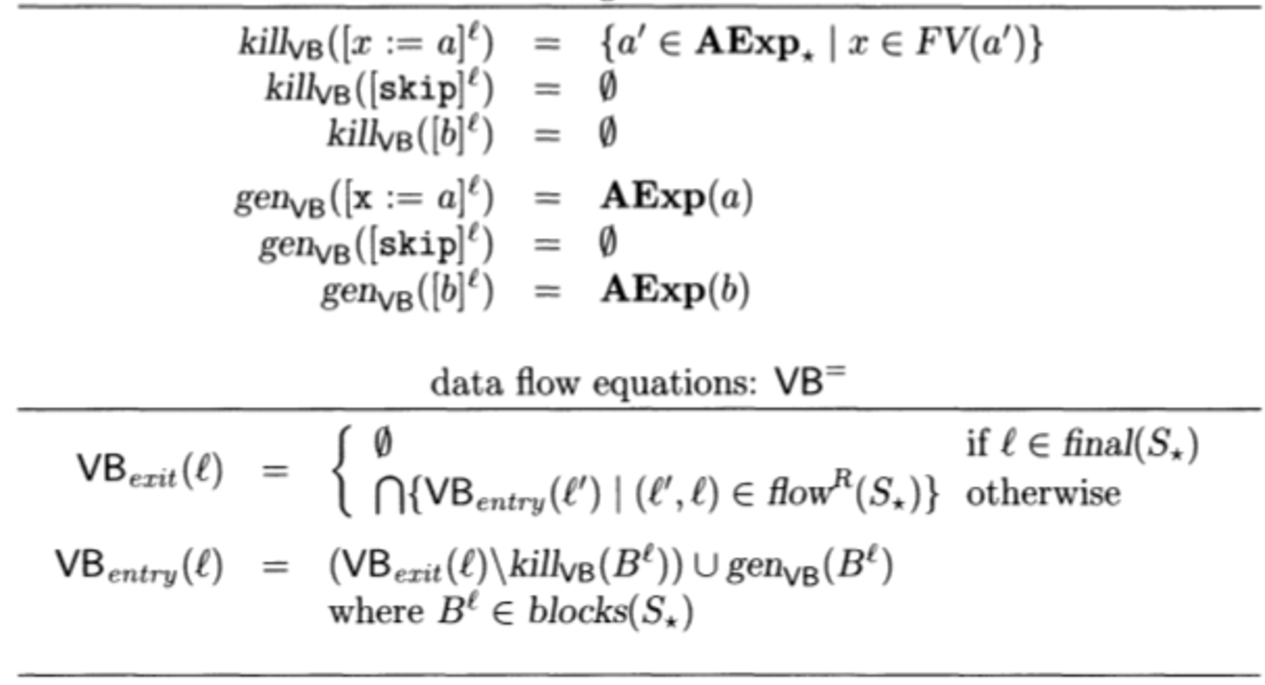
\includegraphics[scale=0.5]{images/vbe}
    \scriptsize{Nielson et al. Principles of Program Analysis. Springer-Verlag. 2005}}
\end{frame}

\begin{frame}[fragile]
	\frametitle{Very Busy Expressions Algorithm}
	
	\begin{block}{Equations}
		\begin{itemize}
			\item $Out(s) = \bigcap_p In(p), p \in successors(s), s \in stmts$
			\item $In(s) = Gen(s) \cup (Out(s) - Kill(s))$  
		\end{itemize}
	\end{block}
	
	\pause
	
	\begin{block}{Iterative algorithm}
          \begin{algorithmic}
            \Procedure{VeryBusyExpression}{CFG}
              \State $U = AExp_* \text{//se of non trivial expressions}$   
              \State $In[End] = \{\}$ 
              \For{$s \leftarrow CFG.V$}
                \State{$In[s] = U$}
              \EndFor
              \While{$\text{not fixed}$}
                 \For{$s \leftarrow CFG.V$}
                    \State{$\text{compute Out[s]}$}
                    \State{$\text{compute In[s]}$}
                  \EndFor
              \EndWhile
              \State {\bf return} $(In, Out)$
          \EndProcedure 
          \end{algorithmic}
	\end{block}
\end{frame}


\begin{frame}[fragile]
    \begin{columns}
    \column[t]{0.5\textwidth}
    Control Flow Graph
    \digraph[scale=0.35]{VbWhile} {
node [fontname = "Handlee"];
edge [fontname = "Handlee"];

start [
 label = "start";
 shape = ellipse; 
];

n1 [
 label = "if(a != b)";
 shape = diamond;
 xlabel="1";
];

n2 [
 label = "x := b - a";
 shape = rect;
 xlabel="2";
];

n3 [
 label = "y := a - b";
 shape = rect;
 xlabel="3";
];

n4 [
 label = "y := b - a";
 shape = rect;
 xlabel="4";
];

n5 [
 label = "a := 0";
 shape = rect;
 xlabel="5";
];

n6 [
 label = "x := a - b";
 shape = rect;
 xlabel="6";
];

end [
 label = "End";
 shape = ellipse; 
];

start -> n1;
n1 -> n2[label = "yes"];
n1 -> n4[label = "no"];
n2 -> n3;
n3 -> end;
n4 -> n5 -> n6;
n6 -> end;


{
rank=same;
n2;n4;
}

{
rank=same;
n3;n6;
}

}
    
    
    \column[t]{0.5\textwidth}
Example 04 (WHILE language)
    
\begin{verbatim}
if(a != b) then  (1)
  x := b - a;    (2)
  y := a - b;    (3)
else    
  y := b - a;    (4) 
  a = 0;         (5) 
  x = a- b;      (6) 
\end{verbatim}
\end{columns}
\end{frame}



\begin{frame}[fragile, t]
	\frametitle{Iteration 0} 
	
	\begin{center}
		\begin{scriptsize}
			\begin{minipage}{8cm}
				\begin{block}{Equations}
					\begin{itemize}
						\item $Out(s) = \bigcap_p In(p), p \in successors(s), s \in stmts$
						\item $In(s) = Gen(s) \cup (Out(s) - Kill(s))$  
					\end{itemize}
				\end{block}
			\end{minipage}
		\end{scriptsize}
	\end{center}
	
	\begin{columns}[T]
		\begin{column}[T]{.5\textwidth}
			\vspace{0pt}
			\digraph[scale=0.35]{VbWhile} {
node [fontname = "Handlee"];
edge [fontname = "Handlee"];

start [
 label = "start";
 shape = ellipse; 
];

n1 [
 label = "if(a != b)";
 shape = diamond;
 xlabel="1";
];

n2 [
 label = "x := b - a";
 shape = rect;
 xlabel="2";
];

n3 [
 label = "y := a - b";
 shape = rect;
 xlabel="3";
];

n4 [
 label = "y := b - a";
 shape = rect;
 xlabel="4";
];

n5 [
 label = "a := 0";
 shape = rect;
 xlabel="5";
];

n6 [
 label = "x := a - b";
 shape = rect;
 xlabel="6";
];

end [
 label = "End";
 shape = ellipse; 
];

start -> n1;
n1 -> n2[label = "yes"];
n1 -> n4[label = "no"];
n2 -> n3;
n3 -> end;
n4 -> n5 -> n6;
n6 -> end;


{
rank=same;
n2;n4;
}

{
rank=same;
n3;n6;
}

}
		\end{column}
		\begin{column}[T]{.5\textwidth}
			\vspace{30pt}    
			\begin{scriptsize}
				\begin{table}[]
					\begin{tabular}{|l|l|l|}
						\hline
						n & IN{[}n{]} & OUT{[}n{]} \\ \hline
						6  & \{ \} & \{ a - b, b - a \}  \\ \hline
						5  & \{ \} & \{ a - b, b - a \}  \\ \hline
						4  & \{ \} & \{ a - b, b - a \}  \\ \hline
						3  & \{ \} & \{ a - b, b - a \}  \\ \hline
						2  & \{ \} & \{ a - b, b - a \} \\ \hline
						1  & \{ \} & \{ \} \\ \hline
					\end{tabular}
				\end{table}   
			\end{scriptsize}
		\end{column}
		%\hfill
		
	\end{columns}
	
\end{frame}



\begin{frame}[fragile, t]
 \frametitle{Iteration 1} 

\begin{center}
\begin{scriptsize}
\begin{minipage}{8cm}
    \begin{block}{Equations}
    \begin{itemize}
        \item $Out(s) = \bigcap_p In(p), p \in successors(s), s \in stmts$
	    \item $In(s) = Gen(s) \cup (Out(s) - Kill(s))$  
    \end{itemize}
    \end{block}
\end{minipage}
\end{scriptsize}
\end{center}

\begin{columns}[T]
\begin{column}[T]{.4\textwidth}
    \vspace{0pt}
    \digraph[scale=0.35]{VbWhile} {
node [fontname = "Handlee"];
edge [fontname = "Handlee"];

start [
 label = "start";
 shape = ellipse; 
];

n1 [
 label = "if(a != b)";
 shape = diamond;
 xlabel="1";
];

n2 [
 label = "x := b - a";
 shape = rect;
 xlabel="2";
];

n3 [
 label = "y := a - b";
 shape = rect;
 xlabel="3";
];

n4 [
 label = "y := b - a";
 shape = rect;
 xlabel="4";
];

n5 [
 label = "a := 0";
 shape = rect;
 xlabel="5";
];

n6 [
 label = "x := a - b";
 shape = rect;
 xlabel="6";
];

end [
 label = "End";
 shape = ellipse; 
];

start -> n1;
n1 -> n2[label = "yes"];
n1 -> n4[label = "no"];
n2 -> n3;
n3 -> end;
n4 -> n5 -> n6;
n6 -> end;


{
rank=same;
n2;n4;
}

{
rank=same;
n3;n6;
}

}
    \end{column}
    \begin{column}[T]{.6\textwidth}
\vspace{30pt}    
	\begin{scriptsize}
	   \begin{table}[]
\begin{tabular}{|l|l|l|}
\hline
n & IN{[}n{]} & OUT{[}n{]} \\ \hline
6  & \{ a - b \} & \{ \} \pause \\ \hline
5  & \{ \} & \{a - b\} \pause \\ \hline
4  & \{ b - a \} & \{ \} \pause \\ \hline
3  & \{ a - b \} & \{ \} \pause \\ \hline
2  & \{ a - b, b - a \} & \{ a - b \}\pause \\ \hline
1  & \{ b - a \} & \{  \}\pause \\ \hline
\end{tabular}
\end{table}   
	\end{scriptsize}
	\end{column}
%\hfill
    
\end{columns}

\end{frame}






















%% \begin{frame}[fragile]
%%     \begin{columns}
%%     \column[t]{0.5\textwidth}
%% Example 05 (Jimple (simplified))
    
%% \begin{verbatim}
%%   if(a = b) goto label1 (1)
%%   x := b - a;           (2)
%%   y := a - b;           (3)
%%   goto label2           (7)
%% label 1:
%%   y := b - a;           (4) 
%%   a = 0;                (5) 
%%   x = a- b;             (6)
%% label 2:
%%   return;               (8)
%% \end{verbatim}

%% \column[t]{0.5\textwidth}
%% Control Flow Graph
%% \digraph[scale=0.35]{VbJimple} {
node [fontname = "Handlee"];
edge [fontname = "Handlee"];

start [
 label = "start";
 shape = ellipse; 
];

n1 [
 label = "if a == b goto label1";
 shape = diamond;
 xlabel="1";
];

n2 [
 label = "x = b - a";
 shape = rect;
 xlabel="2";
];

n3 [
 label = "y = a - b";
 shape = rect;
 xlabel="3";
];

n4 [
 label = "y = b - a";
 shape = rect;
 xlabel="4";
];

n5 [
 label = "a = 0";
 shape = rect;
 xlabel="5";
];

n6 [
 label = "x = a - b";
 shape = rect;
 xlabel="6";
];

n7 [
 label = "goto label2";
 shape = rect;
 xlabel="7";
];

n8 [
 label = "return";
 shape = rect;
 xlabel="8";
];

end [
 label = "End";
 shape = ellipse; 
];

start -> n1;
n1 -> n2[label = "true"];
n1 -> n4[label = "false"];
n2 -> n3 -> n7;
n4 -> n5 -> n6;
n6 -> n8;
n7 -> n8;
n8 -> end;

}
%% \end{columns}
  
%% \end{frame}




%% \begin{frame}[fragile, t]
%%  \frametitle{Iteration 1} 

%% \begin{center}
%% \begin{scriptsize}
%% \begin{minipage}{8cm}
%%     \begin{block}{Equations}
%%     \begin{itemize}
%%         \item $Out(s) = \bigcap_p In(p), p \in successors(s), s \in stmts$
%% 	    \item $In(s) = Gen(s) \cup (Out(s) - Kill(s))$  
%%     \end{itemize}
%%     \end{block}
%% \end{minipage}
%% \end{scriptsize}
%% \end{center}

%% \begin{columns}[T]
%% \begin{column}[T]{.5\textwidth}
%%     \vspace{0pt}
%%     \digraph[scale=0.35]{VbJimple} {
node [fontname = "Handlee"];
edge [fontname = "Handlee"];

start [
 label = "start";
 shape = ellipse; 
];

n1 [
 label = "if a == b goto label1";
 shape = diamond;
 xlabel="1";
];

n2 [
 label = "x = b - a";
 shape = rect;
 xlabel="2";
];

n3 [
 label = "y = a - b";
 shape = rect;
 xlabel="3";
];

n4 [
 label = "y = b - a";
 shape = rect;
 xlabel="4";
];

n5 [
 label = "a = 0";
 shape = rect;
 xlabel="5";
];

n6 [
 label = "x = a - b";
 shape = rect;
 xlabel="6";
];

n7 [
 label = "goto label2";
 shape = rect;
 xlabel="7";
];

n8 [
 label = "return";
 shape = rect;
 xlabel="8";
];

end [
 label = "End";
 shape = ellipse; 
];

start -> n1;
n1 -> n2[label = "true"];
n1 -> n4[label = "false"];
n2 -> n3 -> n7;
n4 -> n5 -> n6;
n6 -> n8;
n7 -> n8;
n8 -> end;

}
%%     \end{column}
%%     \begin{column}[T]{.5\textwidth}
%% \vspace{30pt}    
%% 	\begin{scriptsize}
%% 	   \begin{table}[]
%% \begin{tabular}{|l|l|l|}
%% \hline
%% n & IN{[}n{]} & OUT{[}n{]} \\ \hline
%% 8  & \{ \} & \{ \} \pause \\ \hline
%% 7  & \{ \} & \{ \} \pause \\ \hline
%% 6  & \{ \} & \{ \} \pause \\ \hline
%% 5  & \{ \} & \{ \} \pause \\ \hline
%% 4  & \{ \} & \{ \} \pause \\ \hline
%% 3  & \{ \} & \{ \} \pause \\ \hline
%% 2  & \{ \} & \{ \} \pause \\ \hline
%% 1  & \{ \} & \{ \} \pause \\ \hline
%% \end{tabular}
%% \end{table}   
%% 	\end{scriptsize}
%% 	\end{column}
%% %\hfill
    
%% \end{columns}

%% \end{frame}
